\chapter{Model-Free prediction}

In questa lezione affrontiamo il problema della \textbf{model-free prediction}, ovvero
la stima della funzione valore di una policy \textbf{senza conoscere il modello dell’ambiente}.
In particolare, analizziamo i principali algoritmi di \textit{policy evaluation}:

\begin{compactitemize}
    \item \textbf{Monte Carlo}
    \item \textbf{TD(0)}
    \item \textbf{TD($\lambda$)}
\end{compactitemize}

Il contesto è il seguente: assumiamo di avere una policy fissata $\pi$ e vogliamo stimare
la sua \textbf{state-value function} $v^\pi(s)$ osservando esclusivamente episodi di esperienza
generati seguendo $\pi$.

\section{Monte-Carlo}

I metodi \textbf{Monte Carlo} stimano la funzione valore utilizzando il ritorno
\textit{completo} degli episodi.
Essi non richiedono alcuna conoscenza del modello dell’ambiente e aggiornano le stime
solo dopo che un episodio è terminato.

\noindent
L’obiettivo è:

\[
\text{Reinforcement goal: learn } v^\pi \text{ from episodes of experience under policy } \pi
\]

Osserviamo episodi di esperienza della forma:
\[
S_1, A_1, R_2, \dots, S_T \sim \pi
\]

Ricordiamo che il \textbf{return} a partire dal tempo $t$ è definito come:
\[
G_t = R_{t+1} + \gamma R_{t+2} + \dots + \gamma^{T-1-t} R_T
\]

Il return rappresenta la ricompensa totale scontata che l’agente ottiene a partire dallo
stato $S_t$ fino alla fine dell’episodio.

La \textbf{value function} di una policy $\pi$ è definita come il valore atteso del return:
\[
v^\pi(s) = \mathbb{E}_\pi \left[ G_t \mid S_t = s \right]
\]

Poiché l’aspettativa non è direttamente calcolabile, Monte Carlo policy evaluation
la approssima tramite la \textbf{media empirica dei return osservati}.

\subsection{First-Visit Monte-Carlo}

Nel \textbf{First-Visit Monte-Carlo}, per ciascuno stato $s$ consideriamo solo
la \textbf{prima volta} in cui esso viene visitato all’interno di un episodio.

Per valutare uno stato $s$:

\begin{compactitemize}
    \item identifichiamo il primo time-step $t$ dell’episodio tale che $S_t = s$;
    \item incrementiamo il numero di visite:
    \[
    N(s) \leftarrow N(s) + 1
    \]
    \item accumuliamo il return osservato:
    \[
    S(s) \leftarrow S(s) + G_t
    \]
\end{compactitemize}

La stima del valore è data dalla media:
\[
V(s) = \frac{S(s)}{N(s)}
\]

Grazie alla legge dei grandi numeri, questa stima converge al valore vero:
\[
V(s) \xrightarrow[N(s)\to\infty]{} v^\pi(s)
\]

\subsection{Every-Visit Monte-Carlo}

Nel \textbf{Every-Visit Monte-Carlo}, si utilizza invece \textbf{ogni visita} allo stato $s$
in un episodio, non solo la prima.

Per valutare uno stato $s$:

\begin{compactitemize}
    \item per ogni time-step $t$ tale che $S_t = s$;
    \item incrementiamo il contatore:
    \[
    N(s) \leftarrow N(s) + 1
    \]
    \item accumuliamo il return:
    \[
    S(s) \leftarrow S(s) + G_t
    \]
\end{compactitemize}

Anche in questo caso la stima è la media:
\[
V(s) = \frac{S(s)}{N(s)}
\]

e vale la convergenza:
\[
V(s) \xrightarrow[N(s)\to\infty]{} v^\pi(s)
\]

\noindent
La differenza principale rispetto al First-Visit è che qui alcune visite allo stesso stato
possono contribuire più volte all’apprendimento, riducendo talvolta la varianza
ma introducendo maggiore correlazione tra i campioni.

\subsection{Incremental Mean}

Per calcolare le medie in modo efficiente, senza memorizzare tutti i return osservati,
si utilizza una forma incrementale.

Data una sequenza $x_1, x_2, \dots$, la media:
\[
\mu_k = \frac{1}{k} \sum_{j=1}^{k} x_j
\]

può essere aggiornata come:
\[
\mu_k
=
\mu_{k-1}
+
\frac{1}{k}
\left(
x_k - \mu_{k-1}
\right)
\]

Questa relazione è alla base degli aggiornamenti incrementali Monte Carlo.

\subsection{Incremental Monte-Carlo Policy Evaluation}

Dopo aver osservato un intero episodio:
\[
S_1, A_1, R_2, \dots, S_T
\]

per ciascuno stato $S_t$ visitato con return $G_t$, si aggiornano:

\[
N(S_t) \leftarrow N(S_t) + 1
\]

\[
V(S_t)
\leftarrow
V(S_t)
+
\frac{1}{N(S_t)}
\left(
G_t - V(S_t)
\right)
\]

\noindent
Questo aggiornamento equivale al calcolo incrementale della media dei return
associati allo stato $S_t$.

\subsection{Running Mean in Non-Stationary Problems}

Nei problemi non stazionari, in cui le statistiche dell’ambiente possono cambiare nel tempo,
può essere utile dare più peso alle esperienze recenti.

In questo caso si utilizza uno step-size costante $\alpha$:
\[
V(S_t)
\leftarrow
V(S_t)
+
\alpha
\left(
G_t - V(S_t)
\right)
\]

\noindent
Questa formulazione non converge alla media esatta, ma consente
di adattarsi più rapidamente ai cambiamenti dell’ambiente.

\section{Temporal-Difference Learning}

I metodi di \textbf{Temporal-Difference (TD) Learning} rappresentano una famiglia di algoritmi
model-free che stimano la funzione valore \textit{incrementalmente}, combinando
idee di Monte Carlo e Dynamic Programming.

A differenza dei metodi Monte Carlo, che attendono la fine dell’episodio,
i metodi TD aggiornano le stime \textbf{prima di conoscere l’esito finale},
sfruttando il \textbf{bootstrapping}.

\subsection{From Monte Carlo to Temporal-Difference}

L’obiettivo rimane lo stesso:
\[
\text{learn } v^\pi \text{ from experience under policy } \pi
\]

Nel caso Monte Carlo incrementale, l’aggiornamento è:
\[
V(S_t) \leftarrow V(S_t) + \alpha \big( G_t - V(S_t) \big)
\]

dove il valore viene aggiornato verso il \textit{return reale} $G_t$.
Questo richiede necessariamente la fine dell’episodio.

L’idea chiave di TD è sostituire il return completo con una \textbf{stima del return}.

\subsection{TD(0)}

Il più semplice algoritmo TD è \textbf{TD(0)}.
Invece di usare il return completo, TD(0) utilizza il target:
\[
R_{t+1} + \gamma V(S_{t+1})
\]

L’aggiornamento diventa:
\[
V(S_t) \leftarrow V(S_t)
+
\alpha \Big(
R_{t+1} + \gamma V(S_{t+1}) - V(S_t)
\Big)
\]

Dove:
\begin{compactitemize}
    \item $R_{t+1} + \gamma V(S_{t+1})$ è il \textbf{TD target}
    \item $R_{t+1} + \gamma V(S_{t+1}) - V(S_t)$ è il \textbf{TD error}
\end{compactitemize}

TD può essere visto come un metodo che:
\begin{quote}
\emph{aggiorna una stima verso un’altra stima (potenzialmente migliore)}
\end{quote}

\subsection{Online Learning and Bootstrapping}

Le proprietà fondamentali di TD learning sono:

\begin{compactitemize}
    \item è \textbf{model-free}: non richiede conoscenza di transizioni o reward;
    \item apprende \textbf{online}, dopo ogni singolo step;
    \item apprende anche da \textbf{episodi incompleti};
    \item sfrutta il bootstrapping, usando stime correnti per aggiornare altre stime.
\end{compactitemize}

Questo rende TD particolarmente adatto agli ambienti \textit{continuing}
(non terminanti).

\subsection{Bias--Variance Trade-Off}

Il confronto tra Monte Carlo e TD si spiega naturalmente in termini
di \textbf{bias} e \textbf{varianza}.

Il return Monte Carlo:
\[
G_t = R_{t+1} + \gamma R_{t+2} + \dots + \gamma^{T-1} R_T
\]

è uno stimatore:
\begin{compactitemize}
    \item \textbf{unbiased} di $v^\pi(S_t)$;
    \item ma ad \textbf{alta varianza}, poiché dipende da molte transizioni casuali.
\end{compactitemize}

Il \emph{vero} TD target:
\[
R_{t+1} + \gamma v^\pi(S_{t+1})
\]

sarebbe anch’esso unbiased, ma non è disponibile.

Il TD target utilizzato in pratica:
\[
R_{t+1} + \gamma V(S_{t+1})
\]

è:
\begin{compactitemize}
    \item \textbf{biased} (dipende da una stima);
    \item ma con \textbf{varianza molto più bassa} rispetto a $G_t$.
\end{compactitemize}

\subsection{Advantages and Disadvantages of MC vs TD}

\paragraph{Monte Carlo}
\begin{compactitemize}
    \item zero bias, alta varianza;
    \item buone proprietà di convergenza;
    \item funziona bene anche con function approximation non lineare;
    \item poco sensibile ai valori iniziali;
    \item richiede episodi completi;
    \item applicabile solo a problemi episodici.
\end{compactitemize}

\paragraph{Temporal-Difference}
\begin{compactitemize}
    \item bias non nullo, varianza ridotta;
    \item apprendimento online e incrementale;
    \item può apprendere da sequenze incomplete;
    \item adatto a problemi continuing;
    \item più efficiente in ambienti Markoviani;
    \item più sensibile ai valori iniziali.
\end{compactitemize}

\subsection{Batch Monte Carlo vs Batch TD}

Supponiamo di avere un dataset finito di $K$ episodi:
\[
\{ s_1^k, a_1^k, r_2^k, \dots, s_{T_k}^k \}_{k=1}^K
\]

Ripetendo ciclicamente Monte Carlo o TD(0) sugli episodi:

\begin{compactitemize}
    \item Monte Carlo converge alla soluzione che minimizza il \textbf{mean squared error}
    rispetto ai return osservati:
    \[
    \sum_{k=1}^K \sum_{t=1}^{T_k}
    \big(
    G_t^k - V(s_t^k)
    \big)^2
    \]
    \item TD(0) converge alla soluzione del \textbf{maximum likelihood Markov model}
    che meglio spiega i dati:
    \[
    \hat{P}_{s,s'}^a
    =
    \frac{1}{N(s,a)}
    \sum_{k=1}^K
    \sum_{t=1}^{T_k}
    \mathbf{1}(s_t^k, a_t^k, s_{t+1}^k = s,a,s')
    \]

    \[
    \hat{R}_{s,s'}^{a}
    =
    \frac{1}{N(s,a)}
    \sum_{k=1}^{K}
    \sum_{t=1}^{T_k}
    \mathbf{1}
    \big(
    s_t^{k} = s,\;
    a_t^{k} = a,\;
    s_{t+1}^{k} = s'
    \big)
    \, r_t^{k}
    \]

\end{compactitemize}

\subsection{Certainty Equivalence}

TD learning sfrutta esplicitamente la \textbf{Markov property} dell’ambiente,
mentre Monte Carlo no.

Di conseguenza:
\begin{compactitemize}
    \item TD è generalmente più efficiente negli ambienti Markoviani;
    \item Monte Carlo può essere più efficace in ambienti non Markoviani.
\end{compactitemize}

\section{TD($\lambda$)}
\begin{wrapfigure}{r}{0.3\textwidth}
    \centering
    \vspace{-10pt}
    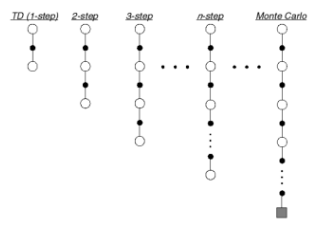
\includegraphics[width=\linewidth]{images/TDL.png}
    \label{fig:TDlambda}
    \vspace{-10pt}
\end{wrapfigure}

L'idea di TD($\lambda$) è quella di costruire un ponte continuo tra TD(0) e Monte Carlo,
combinando informazione a breve termine (pochi passi nel futuro)
e informazione a lungo termine (return completo).
Questo avviene introducendo prima gli \emph{$n$-step return}
e successivamente il \emph{$\lambda$-return}.

\subsection{$n$-step return}

Consideriamo una traiettoria generata sotto una policy $\pi$:
\[
S_1, A_1, R_2, S_2, A_2, R_3, \dots, S_T.
\]

Per lo stato $S_t$ possiamo definire diversi target, a seconda di quanto lontano
nel futuro vogliamo guardare.

Per $n = 1$ otteniamo il target TD(0):
\[
G_t^{(1)} = R_{t+1} + \gamma V(S_{t+1}).
\]

Per $n = 2$:
\[
G_t^{(2)} = R_{t+1} + \gamma R_{t+2} + \gamma^2 V(S_{t+2}).
\]

Per $n = \infty$ (episodio finito) otteniamo il return Monte Carlo:
\[
G_t^{(\infty)} =
R_{t+1} + \gamma R_{t+2} + \dots + \gamma^{T-t-1} R_T.
\]

In generale, l’\textbf{$n$-step return} è:
\[
G_t^{(n)} =
R_{t+1} + \gamma R_{t+2} + \dots + \gamma^{n-1} R_{t+n}
+ \gamma^n V(S_{t+n}),
\]
dove, se l’episodio termina prima, si smette semplicemente di bootstrappare.

L’aggiornamento \textbf{$n$-step TD} è:
\[
V(S_t) \leftarrow V(S_t) + \alpha \left(G_t^{(n)} - V(S_t)\right).
\]

Valori piccoli di $n$ producono target più biased ma a bassa varianza,
valori grandi di $n$ producono target meno biased ma più rumorosi.

\subsection{Media degli $n$-step return}

Invece di scegliere un singolo valore di $n$, possiamo combinare più $n$-step return.
Per esempio:
\[
\frac{1}{2} G_t^{(2)} + \frac{1}{2} G_t^{(4)}.
\]

L’idea generale è sfruttare informazione a diversi orizzonti temporali.
Il problema è farlo in modo teoricamente consistente ed efficiente.
La soluzione è il \textbf{$\lambda$-return}.

\subsection{Il $\lambda$-return}

Il $\lambda$-return combina \emph{tutti} gli $n$-step return con pesi geometrici:
\[
G_t^\lambda
=
(1 - \lambda)\sum_{n=1}^{\infty} \lambda^{n-1} G_t^{(n)},
\qquad 0 \le \lambda \le 1.
\]

I pesi $(1-\lambda)\lambda^{n-1}$ assegnano più importanza agli orizzonti temporali
vicini e riducono progressivamente il contributo di quelli più lontani.

Casi limite:
\begin{compactitemize}
    \item $\lambda = 0 \Rightarrow G_t^\lambda = G_t^{(1)}$ (TD(0));
    \item $\lambda \rightarrow 1 \Rightarrow$ comportamento Monte Carlo.
\end{compactitemize}

L’aggiornamento \textbf{forward-view TD($\lambda$)} è:
\[
V(S_t) \leftarrow V(S_t) + \alpha \left(G_t^\lambda - V(S_t)\right).
\]

\subsection{Forward e Backward View TD($\lambda$)}

La \textbf{forward view} descrive \emph{cosa} TD($\lambda$) sta stimando: la funzione valore viene
aggiornata verso il \textbf{$\lambda$-return} $G_t^\lambda$, che combina tutti gli $n$-step return.
Poiché $G_t^\lambda$ dipende dai reward futuri, questa formulazione richiede episodi completi ed è
quindi concettualmente simile ai metodi Monte Carlo.

La \textbf{backward view} descrive invece \emph{come} implementare TD($\lambda$) in pratica.
Attraverso le \textbf{eligibility traces}, l’errore TD calcolato a ogni passo viene propagato
agli stati visitati in passato, permettendo aggiornamenti \textbf{online} e incrementali, senza
attendere la fine dell’episodio.

In sintesi: la forward view fornisce il significato teorico di TD($\lambda$), mentre la backward view
fornisce il meccanismo computazionale efficiente che rende l’algoritmo utilizzabile in pratica.

\subsection{Eligibility Traces}

Le \textbf{eligibility traces} costituiscono il meccanismo fondamentale della backward view di
TD($\lambda$) e forniscono una soluzione al cosiddetto \emph{credit assignment problem}, ovvero il
problema di determinare quali stati passati siano responsabili di una ricompensa osservata nel
presente. In un processo decisionale sequenziale, una ricompensa tardiva può infatti dipendere da
azioni o stati visitati molto prima, rendendo non banale l’assegnazione del merito.

Due euristiche intuitive emergono naturalmente in questo contesto. La prima è la
\emph{frequency heuristic}, secondo cui gli stati visitati più frequentemente dovrebbero ricevere
maggiore credito. La seconda è la \emph{recency heuristic}, che privilegia invece gli stati visitati
più di recente. Le eligibility traces combinano entrambe le idee, assegnando a ogni stato una traccia
che cresce quando lo stato viene visitato e decade esponenzialmente nel tempo.

Formalmente, a ogni stato $s$ è associata una eligibility trace $E_t(s)$, inizializzata a zero.
Al tempo $t$, la trace viene aggiornata come
\[
E_t(s) = \gamma \lambda E_{t-1}(s) + \mathbb{1}(S_t = s),
\]
dove $\gamma$ è il fattore di sconto, $\lambda \in [0,1]$ controlla la velocità di decadimento della
traccia e $\mathbb{1}(S_t = s)$ vale 1 se lo stato corrente è $s$ e 0 altrimenti. In questo modo, uno
stato visitato di recente avrà una trace elevata, mentre il contributo degli stati più lontani nel
tempo diminuisce progressivamente.

Nella \textbf{backward-view TD($\lambda$)}, l’errore di differenza temporale
\[
\delta_t = R_{t+1} + \gamma V(S_{t+1}) - V(S_t)
\]
viene calcolato a ogni passo temporale e utilizzato per aggiornare il valore di tutti gli stati,
pesando l’aggiornamento con la rispettiva eligibility trace. L’aggiornamento della funzione valore è
dato da
\[
V(s) \leftarrow V(s) + \alpha \, \delta_t \, E_t(s),
\]
dove $\alpha$ è il passo di apprendimento. In questo modo, l’errore corrente viene propagato
all’indietro lungo la sequenza di stati visitati, in misura tanto maggiore quanto più lo stato è stato
frequente e recente.

La backward view può essere interpretata come se, a ogni passo, lo stato successivo $S_{t+1}$ fosse
trattato temporaneamente come uno stato terminale, producendo un aggiornamento immediato simile a TD
a un passo, ma distribuito retroattivamente grazie alle eligibility traces. Questo rende possibile
un apprendimento completamente \emph{online} e incrementale, pur mantenendo l’equivalenza teorica con
la forward view basata sui $\lambda$-return, almeno nel caso tabulare e con opportuni vincoli sui
parametri.

In sintesi, le eligibility traces permettono a TD($\lambda$) di coniugare le proprietà di bassa
varianza dei metodi TD con la capacità dei metodi Monte Carlo di assegnare il merito a intere
sequenze di stati, fornendo un compromesso controllato dal parametro $\lambda$.
\begin{figure}[H]
    \centering
    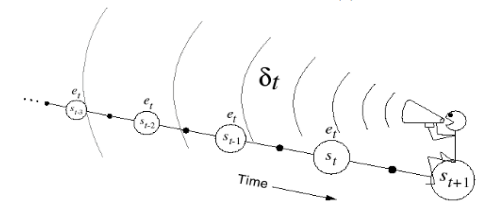
\includegraphics[width=0.6\textwidth]{images/TD2.png}
    \label{fig:student_markov_chain}
\end{figure}
\subsection{TD($\lambda$) e Monte Carlo}

Il parametro $\lambda$ in TD($\lambda$) regola il compromesso tra apprendimento basato su differenze
temporali e apprendimento Monte Carlo, controllando quanto lontano nel tempo venga assegnato il
credito. Al limite $\lambda = 0$, l’algoritmo coincide con TD a un passo, mentre per $\lambda = 1$ si
ottiene un comportamento equivalente ai metodi Monte Carlo nel caso di ambienti episodici e
aggiornamenti \emph{offline}. In quest’ultimo caso, l’aggiornamento effettivo del valore viene infatti
rinviato fino al termine dell’episodio.

L’equivalenza con Monte Carlo può essere compresa osservando l’errore di differenza temporale
$\delta_t = R_{t+1} + \gamma V(S_{t+1}) - V(S_t)$. Per $\lambda = 1$, la somma scontata degli errori TD
a partire da un istante $t$ presenta una proprietà di \emph{telescoping}:
\[
\delta_t + \gamma \delta_{t+1} + \gamma^2 \delta_{t+2} + \cdots + \gamma^{T-1-t} \delta_{T-1},
\]
che, una volta espansa, porta alla cancellazione progressiva dei termini di valore intermedi e si
riduce a
\[
G_t - V(S_t),
\]
dove $G_t$ è il return Monte Carlo. Questo mostra che l’errore totale accumulato da TD(1) su un
episodio coincide esattamente con quello utilizzato dai metodi Monte Carlo.

\subsection{Generalizzazione del telescoping in TD($\lambda$)}

La proprietà di telescoping si estende al caso generale $\lambda \in (0,1)$. In TD($\lambda$), gli
errori di differenza temporale vengono combinati secondo la sequenza
\[
\delta_t + \gamma \lambda \delta_{t+1} + (\gamma \lambda)^2 \delta_{t+2} + \cdots.
\]
Anche in questo caso, l’espansione mostra una cancellazione strutturata dei termini di valore, che
conduce al risultato
\[
G_t^\lambda - V(S_t),
\]
dove $G_t^\lambda$ è il $\lambda$-return della forward view. TD($\lambda$) può quindi essere visto
come un meccanismo che realizza il $\lambda$-return attraverso l’accumulo pesato degli errori TD.

\subsection{Forward e Backward View di TD($\lambda$)}

La relazione tra forward e backward view può essere chiarita considerando un episodio in cui uno
stato $s$ viene visitato una sola volta al tempo $k$. La eligibility trace associata evolve come
\[
E_t(s) =
\begin{cases}
0, & \text{se } t < k, \\
(\gamma \lambda)^{t-k}, & \text{se } t \ge k.
\end{cases}
\]
La backward view accumula gli aggiornamenti online tramite
\[
\sum_{t=1}^{T} \alpha \, \delta_t \, E_t(s)
=
\alpha \sum_{t=k}^{T} (\gamma \lambda)^{t-k} \delta_t,
\]
che, al termine dell’episodio, coincide con
\[
\alpha \bigl(G_k^\lambda - V(S_k)\bigr),
\]
ossia con l’aggiornamento della forward view basato sul $\lambda$-return. Nel caso di visite multiple
allo stesso stato, gli effetti delle diverse visite si sommano naturalmente attraverso le eligibility
traces.

\subsection{Equivalenza Offline e Online}

Nel regime di aggiornamenti \emph{offline}, in cui la funzione valore viene aggiornata solo al termine
dell’episodio, la forward view e la backward view di TD($\lambda$) sono perfettamente equivalenti e
producono identici aggiornamenti complessivi.

Nel regime \emph{online}, invece, gli aggiornamenti vengono applicati a ogni passo temporale. In
questo caso, la backward view costituisce un’approssimazione computazionalmente efficiente della
forward view, ma le due formulazioni non sono più esattamente identiche a causa della modifica
continua delle stime di valore durante l’episodio. Esistono tuttavia varianti, come l’\emph{exact
online TD($\lambda$)}, che ristabiliscono un’equivalenza completa anche nel caso online mediante una
definizione modificata delle eligibility traces.

\begin{figure}[H]
    \centering
    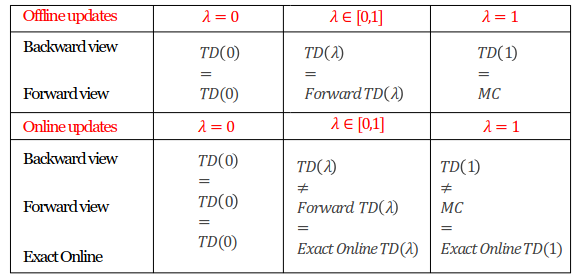
\includegraphics[width=0.9\textwidth]{images/TD3.png}
    \label{fig:student_markov_chain}
\end{figure}